% !Mode:: "TeX:UTF-8"
% !TEX program  = xelatex

\section{一些样例}

以下,笔者结合自己的使用习惯和经验添加了一些内容。
\subsection{图片}

如图\ref{fig.test_figure},是一张测试图片。
\begin{figure}[htb]
    \centering
    \includegraphics[width=.5\textwidth]{example-image-a}
    \caption{自带测试图片---Test image}\label{fig.test_figure}
    % 图片的标题应该在下方
\end{figure}

如图\ref{fig.shu_and_kun},是一只鼠鼠和一值坤坤。如图\ref{fig.shushu},是一只鼠鼠。如图\ref{fig.kunkun},是一只坤坤。

\begin{figure}[htb]
    \centering
    \begin{subfigure}[t]{.35\textwidth}
        \centering
        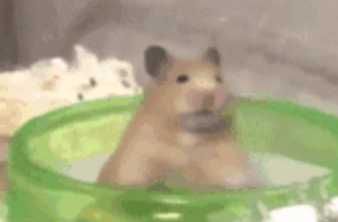
\includegraphics[width=1\textwidth]{figures/shushu.png}
        \caption{这是一只鼠鼠}\label{fig.shushu}
    \end{subfigure}
    \begin{subfigure}[t]{.35\textwidth}
        \centering
        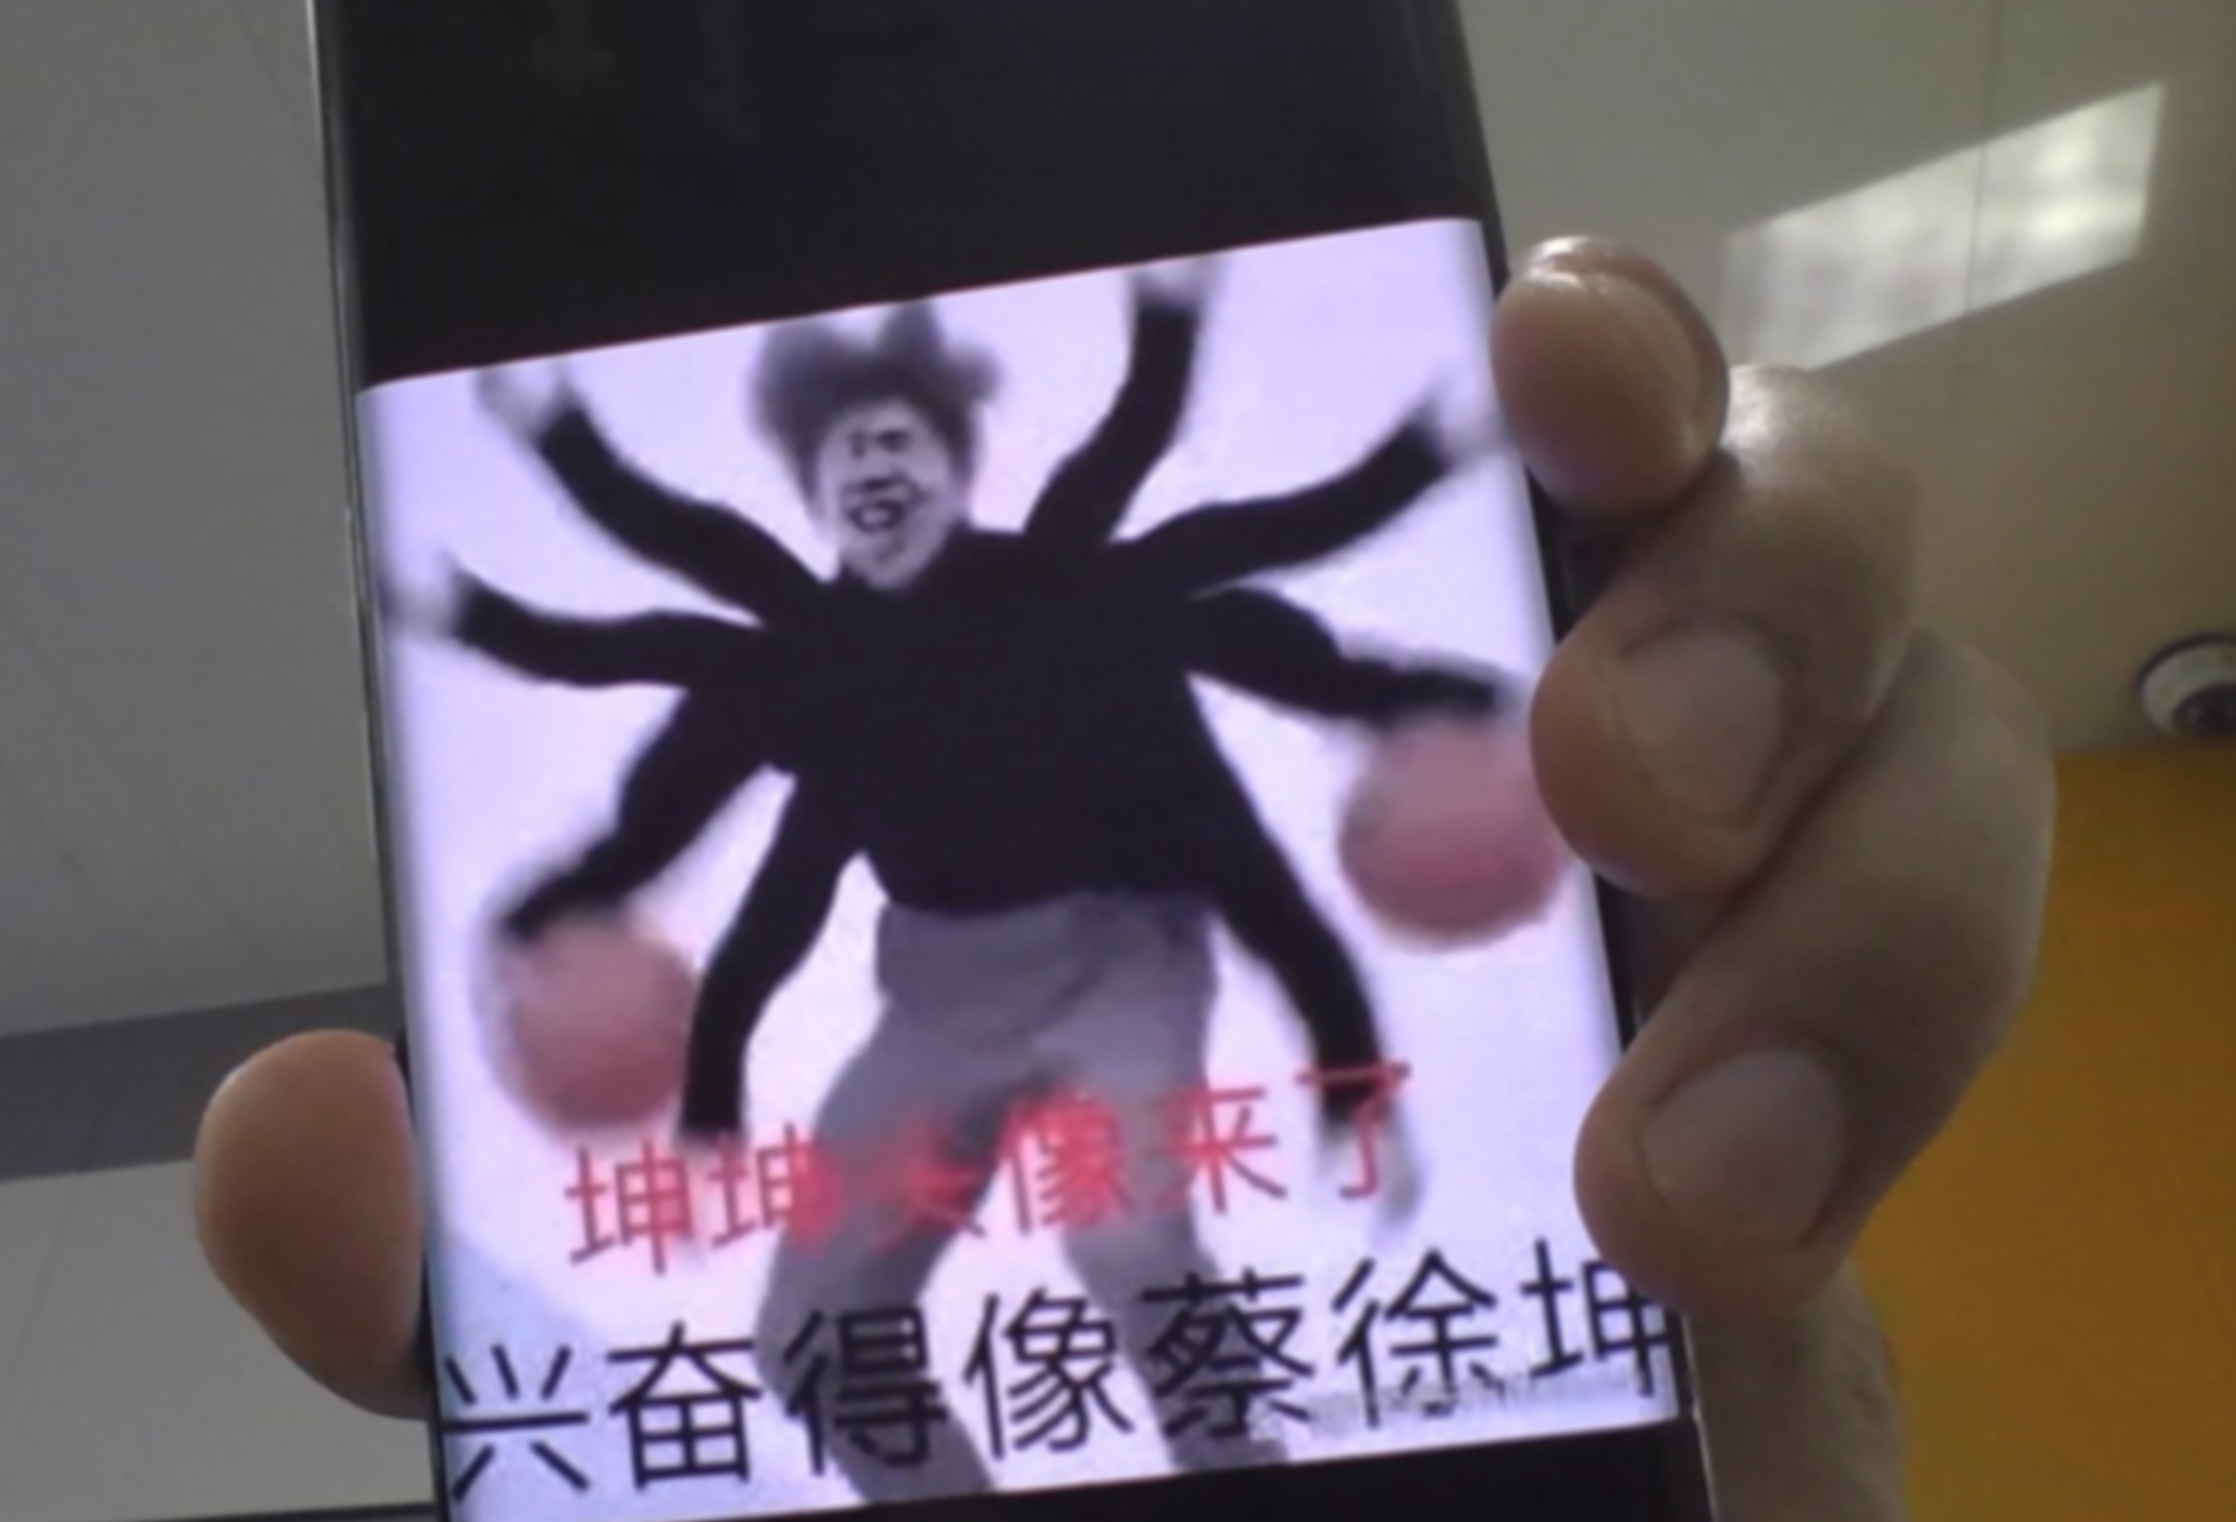
\includegraphics[width=1\textwidth]{figures/kunkun.png}
        \caption{这是一只坤坤,他在说只因你太美,baby}\label{fig.kunkun}
    \end{subfigure}

    \caption{鼠鼠和坤坤}\label{fig.shu_and_kun}
\end{figure}

\subsection{公式}

公式推荐使用\verb|\begin{equation}...\end{equation}|  和\verb|\begin{align}...\end{align}|包裹。在align环境中,不需要标明的公式号的行在末尾处要添加\verb|\nonumber|


示例如下:

\begin{equation}
    \mathbf{M}\begin{pmatrix}\ddot{\mathbf{q}}_f\\\ddot{\mathbf{q}}_j\end{pmatrix}+\mathbf{h}(\mathbf q,\mathbf {\dot q})+\mathbf{g}=\begin{pmatrix}\mathbf{0}_6\\\boldsymbol{\tau}\end{pmatrix}+\boldsymbol{J}_c^\top\mathbf{f}_r
\end{equation}

\begin{align}
    J   & =  ||\Delta \mathbf f||^2_{\mathbf{Q_1}} + ||\Delta \mathbf b||^2_{\mathbf{Q_1}} 
                                \nonumber \\ 
        & =  \begin{bmatrix}
            \Delta \mathbf f \\
            \Delta \mathbf b \\
        \end{bmatrix}^\intercal 
        \begin{bmatrix}
            \mathbf{Q_1} & \\
            & \mathbf{Q_2} \\
        \end{bmatrix}
        \begin{bmatrix}
            \Delta \mathbf f \\
            \Delta \mathbf b \\
        \end{bmatrix} 
                               \nonumber  \\
        & =  \mathbf{u}^\intercal \mathbf H \mathbf{u} + 2\mathbf{u}^\intercal\mathbf h
\end{align}


\subsection{表格}

表格与图片可以直接通过\verbbox{\ref{<key>}}来引用,例如表\ref{table2}、图\ref{F:test-a}、图\ref{F:test-b-sub-b}。

\begin{table}[htb]
% h-here,t-top,b-bottom,优先级依次下降
    % 居中,模版已设定表格浮动体居中
    \centering
    \caption{表格的标题应该放在上方}
    \label{table}
    \begin{tabular}{lc} % 三线表不能有竖线,l-left,c-center,r-right
        \toprule
        %三线表-top 线
        Example & Result \\
        \midrule
        %三线表-middle 线
        Example1          & 0.25 \\
        Example2          & 0.36 \\
        \bottomrule
        %三线表-底线
    \end{tabular}
\end{table}

\begin{table}[htb]
    \centering
    \caption{带表注的表格的标题}
    \label{table2}
    \begin{threeparttable}
        \setlength{\tabcolsep}{0.6cm}{ % 调节表格长度
                \begin{tabular}{lc} % 三线表不能有竖线,l-left,c-center,r-right
                    \toprule
                    %三线表-top 线
                    Example & Result \\
                    \midrule
                    %三线表-middle 线
                    Example1          & 0.25\tnote{1} \\
                    Example2          & 0.36 \\
                    \bottomrule
                    %三线表-底线
                \end{tabular}
        }
        \begin{tablenotes}
            \item[1] 数据来源:南方科技大学 \LaTeX 模版 % 增加表格数据来源注释
        \end{tablenotes}
    \end{threeparttable}
\end{table}

\subsection{参考文献}

参考文献一般使用\verbbox{\cite{<key>}}命令,效果如是\cite{Nicholas1998Handbook},sustechthesis\cite{sustechthesis}。引用作者使用\verbbox{\citeauthor{<key>}},效果如是“\citeauthor{goossens1994latex}”。
